\documentclass[12pt,a4paper]{article}
\usepackage[utf8]{inputenc}
\usepackage{geometry}
\geometry{margin=1in}
\usepackage{amsmath}
\usepackage{amssymb}
\usepackage{graphicx}
\usepackage{hyperref}
\usepackage{setspace}
\usepackage{enumitem}
\usepackage{booktabs}
\usepackage{float}
\usepackage{tikz}
\usetikzlibrary{arrows.meta, positioning, shapes.geometric}
\setstretch{1.3}

\title{Sistem Deteksi Hipoksia Janin Berbasis ResNet Multimodal}
\author{Tim Penelitian HipoxiaDeepLearning}
\date{September 2025}

\begin{document}
\maketitle

\begin{abstract}
Hipoksia janin intrapartum menjadi salah satu penyebab utama morbiditas dan mortalitas perinatal. Penelitian ini menyajikan sistem deteksi hipoksia janin berbasis \textit{deep learning} yang mengintegrasikan sinyal \textit{fetal heart rate} (FHR) dan 26 parameter klinis dari database CTU-UHB (PSYCONET 1.0.0). Fokus utama diarahkan pada arsitektur Residual Network (ResNet) multimodal dengan blok residual tunggal, \textit{global average pooling}, dan mekanisme atensi untuk fusi fitur. Pipeline mencakup konversi data \texttt{.dat/.hea} ke representasi sinyal \texttt{.npy} dan tabular klinis, strategi augmentasi untuk mengatasi ketidakseimbangan kelas, serta evaluasi berbasis metrik klasifikasi dan visualisasi interpretatif. Model mencapai akurasi uji 0.7895 dengan \textit{weighted} F1 0.80 dan menyediakan panel interpretasi visual untuk mendukung pengambilan keputusan obstetri.
\end{abstract}

\tableofcontents
\newpage

\section{Bab 1: Pendahuluan}
\subsection{Latar Belakang}
Deteksi dini hipoksia janin selama persalinan merupakan prioritas klinis karena keterlambatan intervensi dapat menimbulkan asfiksia neonatus, kerusakan neurologis, hingga kematian perinatal\textsuperscript{[1]}. Cardiotocography (CTG) telah lama menjadi standar pemantauan, namun interpretasi manual menunjukkan variabilitas antar klinisi dan akurasi terbatas terutama pada pola borderline\textsuperscript{[2]}. Digitalisasi sinyal CTG dan metadata klinis di database CTU-UHB (PSYCONET 1.0.0) menyediakan 552 rekaman berdurasi 90 menit dengan frekuensi sampling 4 Hz dan outcome pH darah, skor Apgar, serta parameter obstetri-maternal yang terdokumentasi dalam pasangan berkas \texttt{.dat/.hea}.

Residual Network (ResNet) menawarkan kemampuan mempertahankan gradien pada jaringan yang dalam melalui \textit{skip connection}, menjadikannya kandidat kuat untuk mengekstraksi pola kompleks dari sinyal FHR yang panjang\textsuperscript{[3]}. Implementasi pada repositori ini menempatkan ResNet sebagai tulang punggung cabang sinyal dengan blok residual tunggal, \textit{global pooling}, serta cabang klinis berbasis dense layer dan mekanisme atensi.

\subsection{Rumusan Masalah}
\begin{enumerate}[label=\alph*)]
    \item Bagaimana merancang pipeline konversi CTU-UHB dari berkas \texttt{.dat/.hea} menjadi sinyal \texttt{.npy} dan tabular klinis siap latih?
    \item Bagaimana memformulasikan arsitektur ResNet multimodal yang stabil untuk sinyal FHR sepanjang 5.000 sampel dengan integrasi fitur klinis?
    \item Bagaimana kinerja model terhadap metrik klasifikasi utama dan apa implikasinya bagi praktik obstetri?
\end{enumerate}

\subsection{Tujuan Penelitian}
\begin{enumerate}[label=\alph*)]
    \item Mengembangkan prosedur ekstraksi sinyal dan metadata klinis yang terstandar dari dataset PhysioNet.
    \item Mendesain arsitektur ResNet multimodal lengkap dengan landasan matematis residual block dan mekanisme atensi.
    \item Mengevaluasi performa model melalui metrik klasifikasi dan analisis visual serta menafsirkan relevansinya bagi keputusan klinis.
\end{enumerate}

\subsection{Batasan Masalah}
\begin{enumerate}[label=\alph*)]
    \item Studi dibatasi pada sinyal FHR dan 26 parameter klinis; sinyal kontraksi uterus tidak dimodelkan secara eksplisit.
    \item Analisis diarahkan eksklusif pada varian ResNet dalam repositori, tanpa perbandingan dengan metode lain.
    \item Evaluasi dilakukan pada data retrospektif dengan pembagian train/val/test internal; validasi prospektif menjadi pekerjaan lanjutan.
\end{enumerate}

\section{Bab 2: Landasan Teori}
\subsection{Dataset CTU-UHB (PSYCONET 1.0.0)}
Setiap rekaman terdiri dari berkas sinyal \texttt{.dat} dan header \texttt{.hea} yang memuat outcome neonatus (pH, BDecf, pCO\textsubscript{2}, skor Apgar) serta faktor maternal (umur, paritas, diabetes). Informasi kurasi dataset tersaji di \texttt{processed\_data/signal\_info.csv} yang memuat nama berkas, frekuensi sampling 4 Hz, durasi, jumlah sampel, dan kategori pH.

\subsection{Konversi Berkas ke Representasi \texttt{.npy}}
Alur konversi data mengikuti langkah berurutan sebagaimana divisualisasikan pada Gambar~\ref{fig:conversion-flow}. Tahapan tersebut dirangkum sebagai berikut.
\begin{enumerate}[label=\arabic*)]
    \item \textbf{Ekstraksi metadata}. Berkas \texttt{.hea} dibaca untuk memperoleh outcome neonatus, faktor maternal, dan rentang waktu persalinan; nilai kategorikal diubah menjadi numerik dan dilakukan imputasi median yang disesuaikan per label untuk pH.
    \item \textbf{Pemetaan identitas}. Setiap baris metadata diberi \textit{record id} berurutan (1001--1552) agar terhubung dengan berkas sinyal.
    \item \textbf{Pembersihan numerik}. Nilai ekstrim di-clipping pada rentang tiga simpangan baku, sementara kolom klinis lainnya diisi median global untuk meminimalkan data hilang.
    \item \textbf{Pembacaan sinyal}. Pasangan berkas \texttt{.dat} dibaca dan kanal FHR dipisahkan, disertai informasi frekuensi sampling 4 Hz.
    \item \textbf{Normalisasi sinyal}. Sinyal diklip pada rentang fisiologis 50--200 bpm, diseragamkan panjangnya menjadi 5.000 sampel melalui interpolasi atau down-sampling, lalu dinormalisasi menggunakan median dan MAD agar robust terhadap artefak.
    \item \textbf{Penyelarasan multimodal}. Sinyal terproses dan vektor klinis digabungkan dalam struktur \texttt{numpy} sehingga siap dibagi menjadi train/val/test.
\end{enumerate}

\begin{figure}[H]
    \centering
    \tikzset{process/.style={rectangle, rounded corners, minimum width=4.5cm, minimum height=1cm, text centered, draw=black, fill=gray!10}}
    \tikzset{arrow/.style={thick, ->, >=Stealth}}
    \begin{tikzpicture}[node distance=1.6cm]
        \node (start) [process] {Header \texttt{.hea}};
        \node (meta) [process, below=of start] {Ekstraksi metadata \& imputasi label-spesifik};
        \node (map) [process, below=of meta] {Pemetaan \textit{record id} \& clipping outlier};
        \node (signal) [process, below=of map] {Baca sinyal FHR dari \texttt{.dat}};
        \node (norm) [process, below=of signal] {Penyeragaman panjang \& normalisasi median--MAD};
        \node (merge) [process, below=of norm] {Penggabungan sinyal \& fitur klinis};
        \node (end) [process, below=of merge] {Dataset multimodal siap latih};
        \draw [arrow] (start) -- (meta);
        \draw [arrow] (meta) -- (map);
        \draw [arrow] (map) -- (signal);
        \draw [arrow] (signal) -- (norm);
        \draw [arrow] (norm) -- (merge);
        \draw [arrow] (merge) -- (end);
    \end{tikzpicture}
    \caption{Alur konversi data CTU-UHB dari berkas \texttt{.dat/.hea} menjadi sinyal \texttt{.npy} dan tabular klinis.}
    \label{fig:conversion-flow}
\end{figure}

\subsection{Arsitektur ResNet Multimodal}
Gambar~\ref{fig:resnet-architecture} menampilkan ringkasan arsitektur ResNet multimodal yang dibangun pada proyek ini. Implementasi mengikuti langkah-langkah berikut tanpa menayangkan kode secara eksplisit:
\begin{enumerate}[label=\alph*)]
    \item \textbf{Cabang sinyal}. Sinyal FHR satu dimensi di-reshape menjadi tensor $(5000 \times 1)$, kemudian melewati konvolusi awal (64 filter, kernel 31) dengan aktivasi ReLU, batch normalization, dan max pooling ukuran 8 untuk mengekstraksi pola temporal makro.
    \item \textbf{Blok residual}. Output konvolusi awal memasuki dua lapis \textit{Conv1D} berfilter 128 (kernel 15) yang dibungkus batch normalization. Jalur utama dijumlahkan dengan proyeksi \textit{skip connection} (konvolusi $1\times1$) sehingga gradien tetap stabil saat jaringan diperdalam.
    \item \textbf{Pemerataan informasi}. Setelah residual block dilakukan max pooling tambahan dan \textit{global average pooling} untuk mereduksi dimensi menjadi vektor 128 yang mewakili keseluruhan sinyal.
    \item \textbf{Cabang klinis}. Parameter klinis (27 kolom) melewati tiga dense layer berukuran 48--32--16 dengan aktivasi ReLU, batch normalization, dan dropout terkontrol guna menjaga generalisasi.
    \item \textbf{Fusi dan atensi}. Kedua vektor (sinyal dan klinis) digabungkan, dilalui lapisan atensi penuh untuk memberi bobot adaptif terhadap fitur gabungan, kemudian diproses oleh rangkaian dense 144--96--48--32 dengan dropout menurun.
    \item \textbf{Klasifikasi akhir}. Lapisan softmax tiga neuron menghasilkan probabilitas kelas normal, suspect, dan hipoksia. Pelatihan memakai Adam $(6\times10^{-4})$ dengan \textit{early stopping} dan \textit{ReduceLROnPlateau} untuk stabilitas.
\end{enumerate}

\begin{figure}[H]
    \centering
    \tikzset{block/.style={rectangle, rounded corners, draw=black, fill=white, minimum width=2.1cm, minimum height=0.9cm, align=center, inner sep=3pt}}
    \tikzset{arrow/.style={thick, ->, >=Stealth}}
    \begin{tikzpicture}[node distance=1.5cm]
        \node (input) [block] {Input FHR\\$5000\times1$};
        \node (conv) [block, right=of input, text width=2.3cm] {Conv1D 64\\Kernel 31\\BN + ReLU\\MaxPool};
        \node (res) [block, right=of conv, text width=2.4cm] {Residual Block\\Conv1D 128 ($\times2$)\\Skip $1\times1$ + BN};
        \node (gap) [block, right=of res, text width=2.3cm] {MaxPool\\Global Avg Pool\\Dense 128-64};
        \node (clin) [block, below=of res, text width=2.3cm] {Input klinis\\Dense 48-32-16\\BN + Dropout};
        \node (fusion) [block, below=of gap, text width=2.6cm] {Concatenate\\Attention\\Dense 144-96-48-32};
        \node (softmax) [block, below=of fusion, text width=2.1cm] {Softmax\\3 kelas};
        \draw [arrow] (input) -- (conv);
        \draw [arrow] (conv) -- (res);
        \draw [arrow] (res) -- (gap);
        \draw [arrow] (clin) -- (fusion);
        \draw [arrow] (gap) -- (fusion);
        \draw [arrow] (fusion) -- (softmax);
    \end{tikzpicture}
    \caption{Skema arsitektur ResNet multimodal: cabang sinyal mengekstraksi pola FHR, cabang klinis memproses metadata, keduanya digabung dengan mekanisme atensi sebelum klasifikasi.}
    \label{fig:resnet-architecture}
\end{figure}

Fungsi kerugian \textit{focal loss} dan metrik evaluasi klasik (akurasi, precision, recall, F1, ROC) melengkapi landasan teoritis yang digunakan untuk menilai performa.

\section{Bab 3: Metodologi Penelitian}
\subsection{Desain Sistem}
Sistem modular pada berkas \texttt{main\_modular.py} mengorkestrasi modul DataHandler, ModelBuilder, ModelTrainer, Visualizer, dan Interface untuk menjalankan pipeline end-to-end: persiapan data, pelatihan ResNet, evaluasi, serta penyajian analisis prediksi.

\subsection{Akuisisi dan Persiapan Data}
\begin{itemize}
    \item Mengunduh 552 rekaman CTG dari PhysioNet dan memvalidasi 506 sampel dengan sinyal FHR lengkap.
    \item Melakukan konversi sinyal serta penyusunan metadata klinis dan sinyal sebagaimana ditunjukkan pada Gambar~\ref{fig:conversion-flow}.
    \item Membagi dataset secara stratifikasi menjadi 354/76/76 untuk train/val/test.
    \item Menyeimbangkan kelas melalui augmentasi sinyal (penambahan noise, \textit{time shifting}) dan SMOTE-Tomek hingga tiap kelas memiliki 243 sampel.
\end{itemize}

\subsection{Konfigurasi Model dan Pelatihan}
ResNet multimodal dibangun dengan 449.827 parameter. Optimizer Adam menggunakan laju belajar awal \(6 \times 10^{-4}\) untuk stabilitas residual block. \textit{Early stopping} (\textit{patience} 30) dan \textit{ReduceLROnPlateau} (\textit{patience} 12) digunakan untuk mencegah \textit{overfitting}. Bobot kelas hipoksia dinaikkan 1.5 kali guna meningkatkan sensitivitas terhadap kasus kritis.

\subsection{Evaluasi dan Visualisasi}
Setelah pelatihan, sistem menghasilkan laporan evaluasi, menyimpan model dalam format PKL, dan memproduksi 12 grafik pelatihan serta 12 panel interpretasi prediksi. Gambar~\ref{fig:training-loss} dan Gambar~\ref{fig:training-accuracy} menampilkan dinamika loss dan akurasi. Gambar~\ref{fig:confusion-matrix} dan Gambar~\ref{fig:roc-curves} menggambarkan performa klasifikasi pada data uji. Panel interpretasi untuk satu rekaman uji disajikan pada Gambar~\ref{fig:prediction-summary}, Gambar~\ref{fig:prediction-importance}, dan Gambar~\ref{fig:prediction-uncertainty}.

\begin{figure}[H]
    \centering
    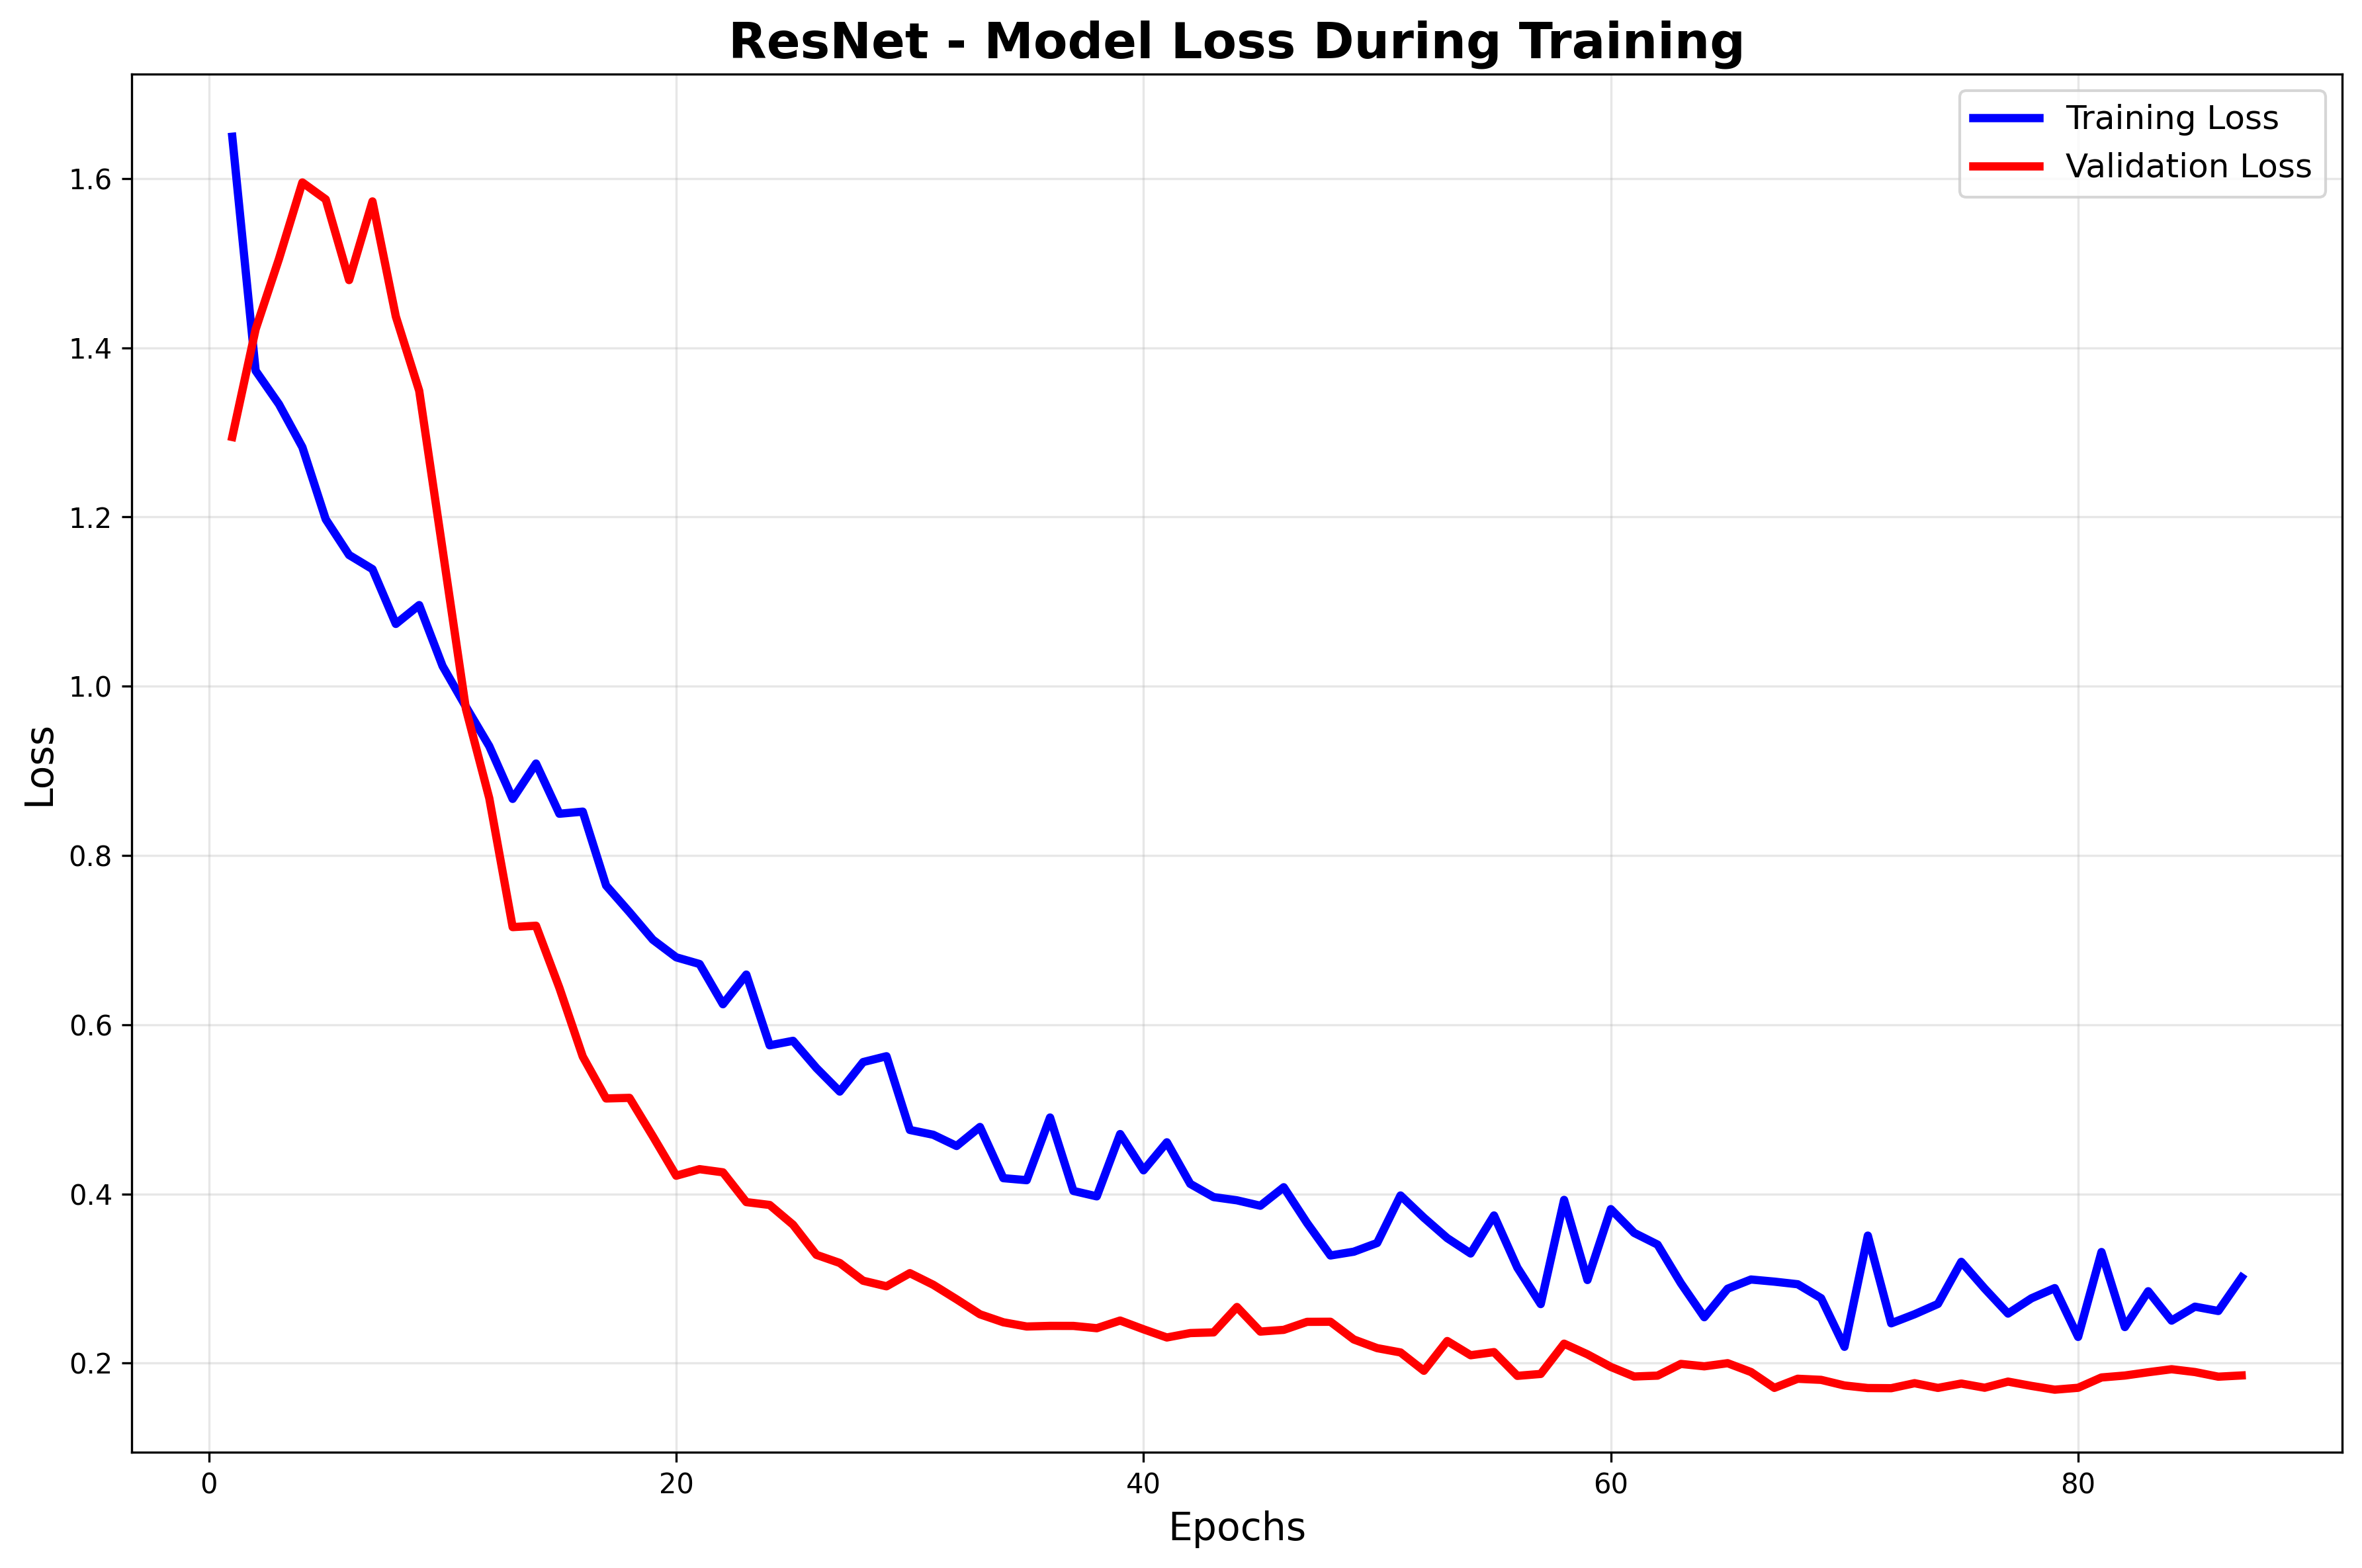
\includegraphics[width=0.85\textwidth]{../results/training_plots/trainingResultResNetMethod/01_training_loss.png}
    \caption{Kurva loss model ResNet selama pelatihan.}
    \label{fig:training-loss}
\end{figure}

\begin{figure}[H]
    \centering
    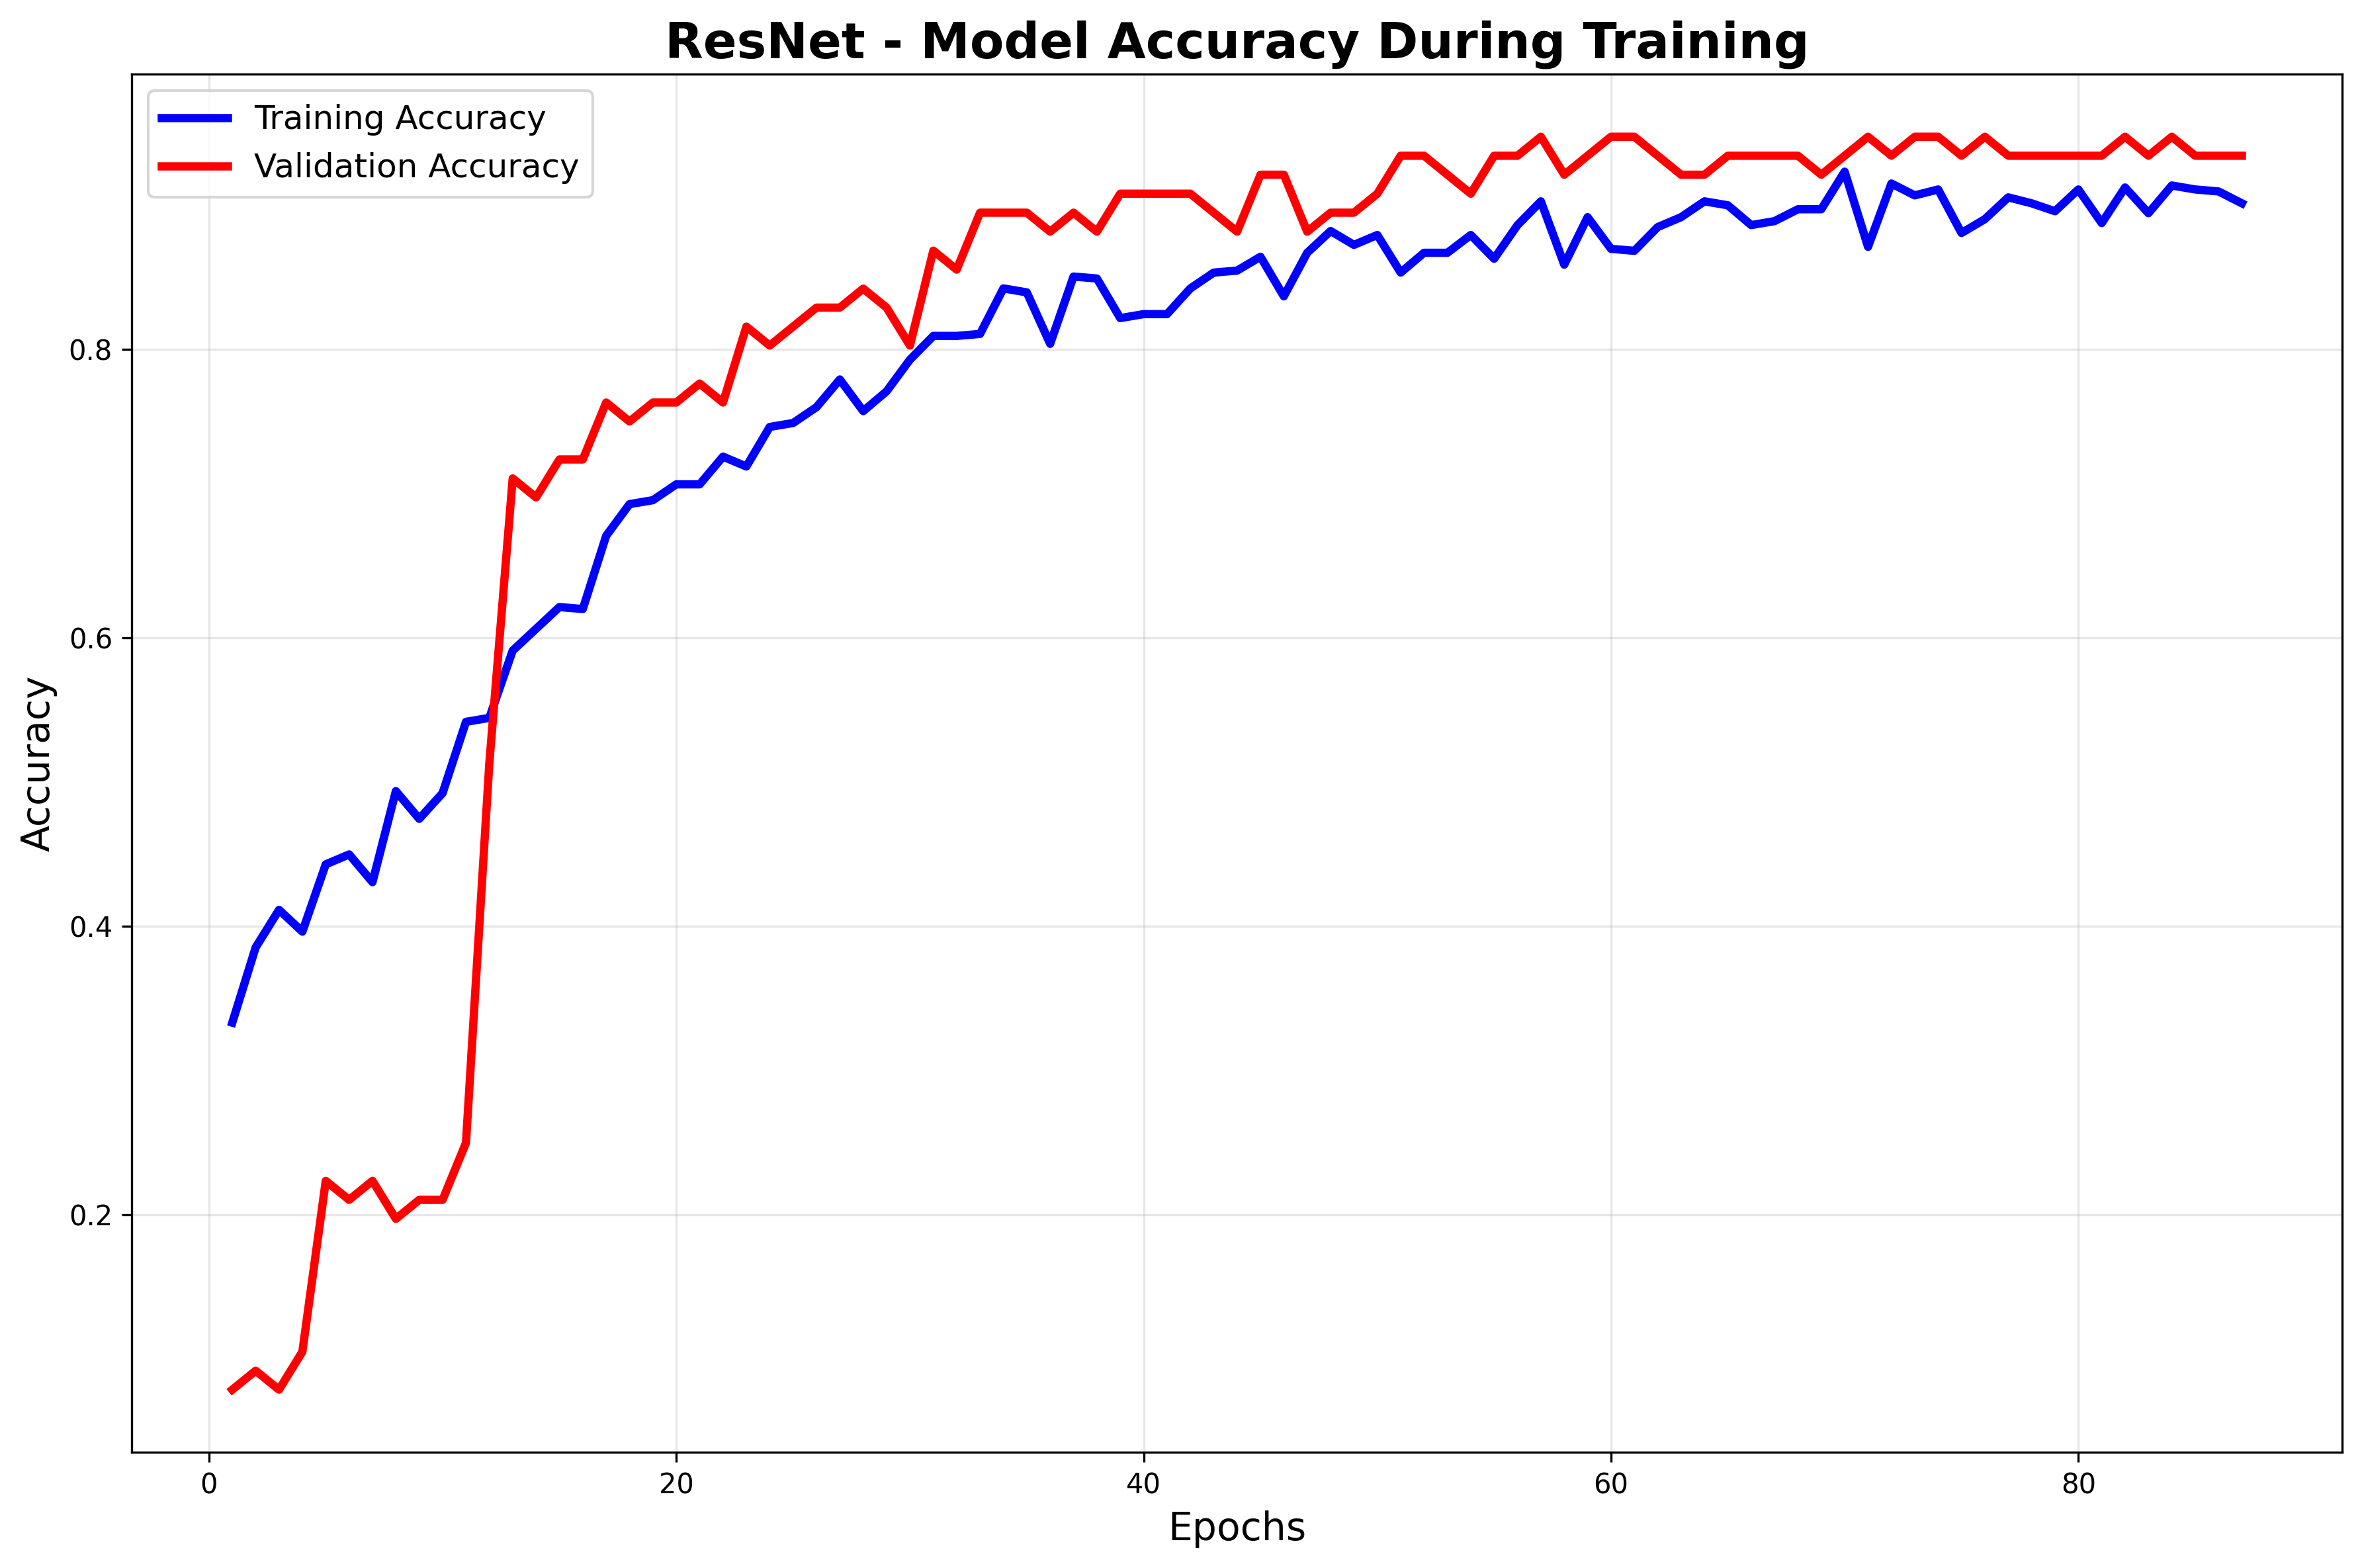
\includegraphics[width=0.85\textwidth]{../results/training_plots/trainingResultResNetMethod/02_training_accuracy.png}
    \caption{Kurva akurasi model ResNet selama pelatihan.}
    \label{fig:training-accuracy}
\end{figure}

\begin{figure}[H]
    \centering
    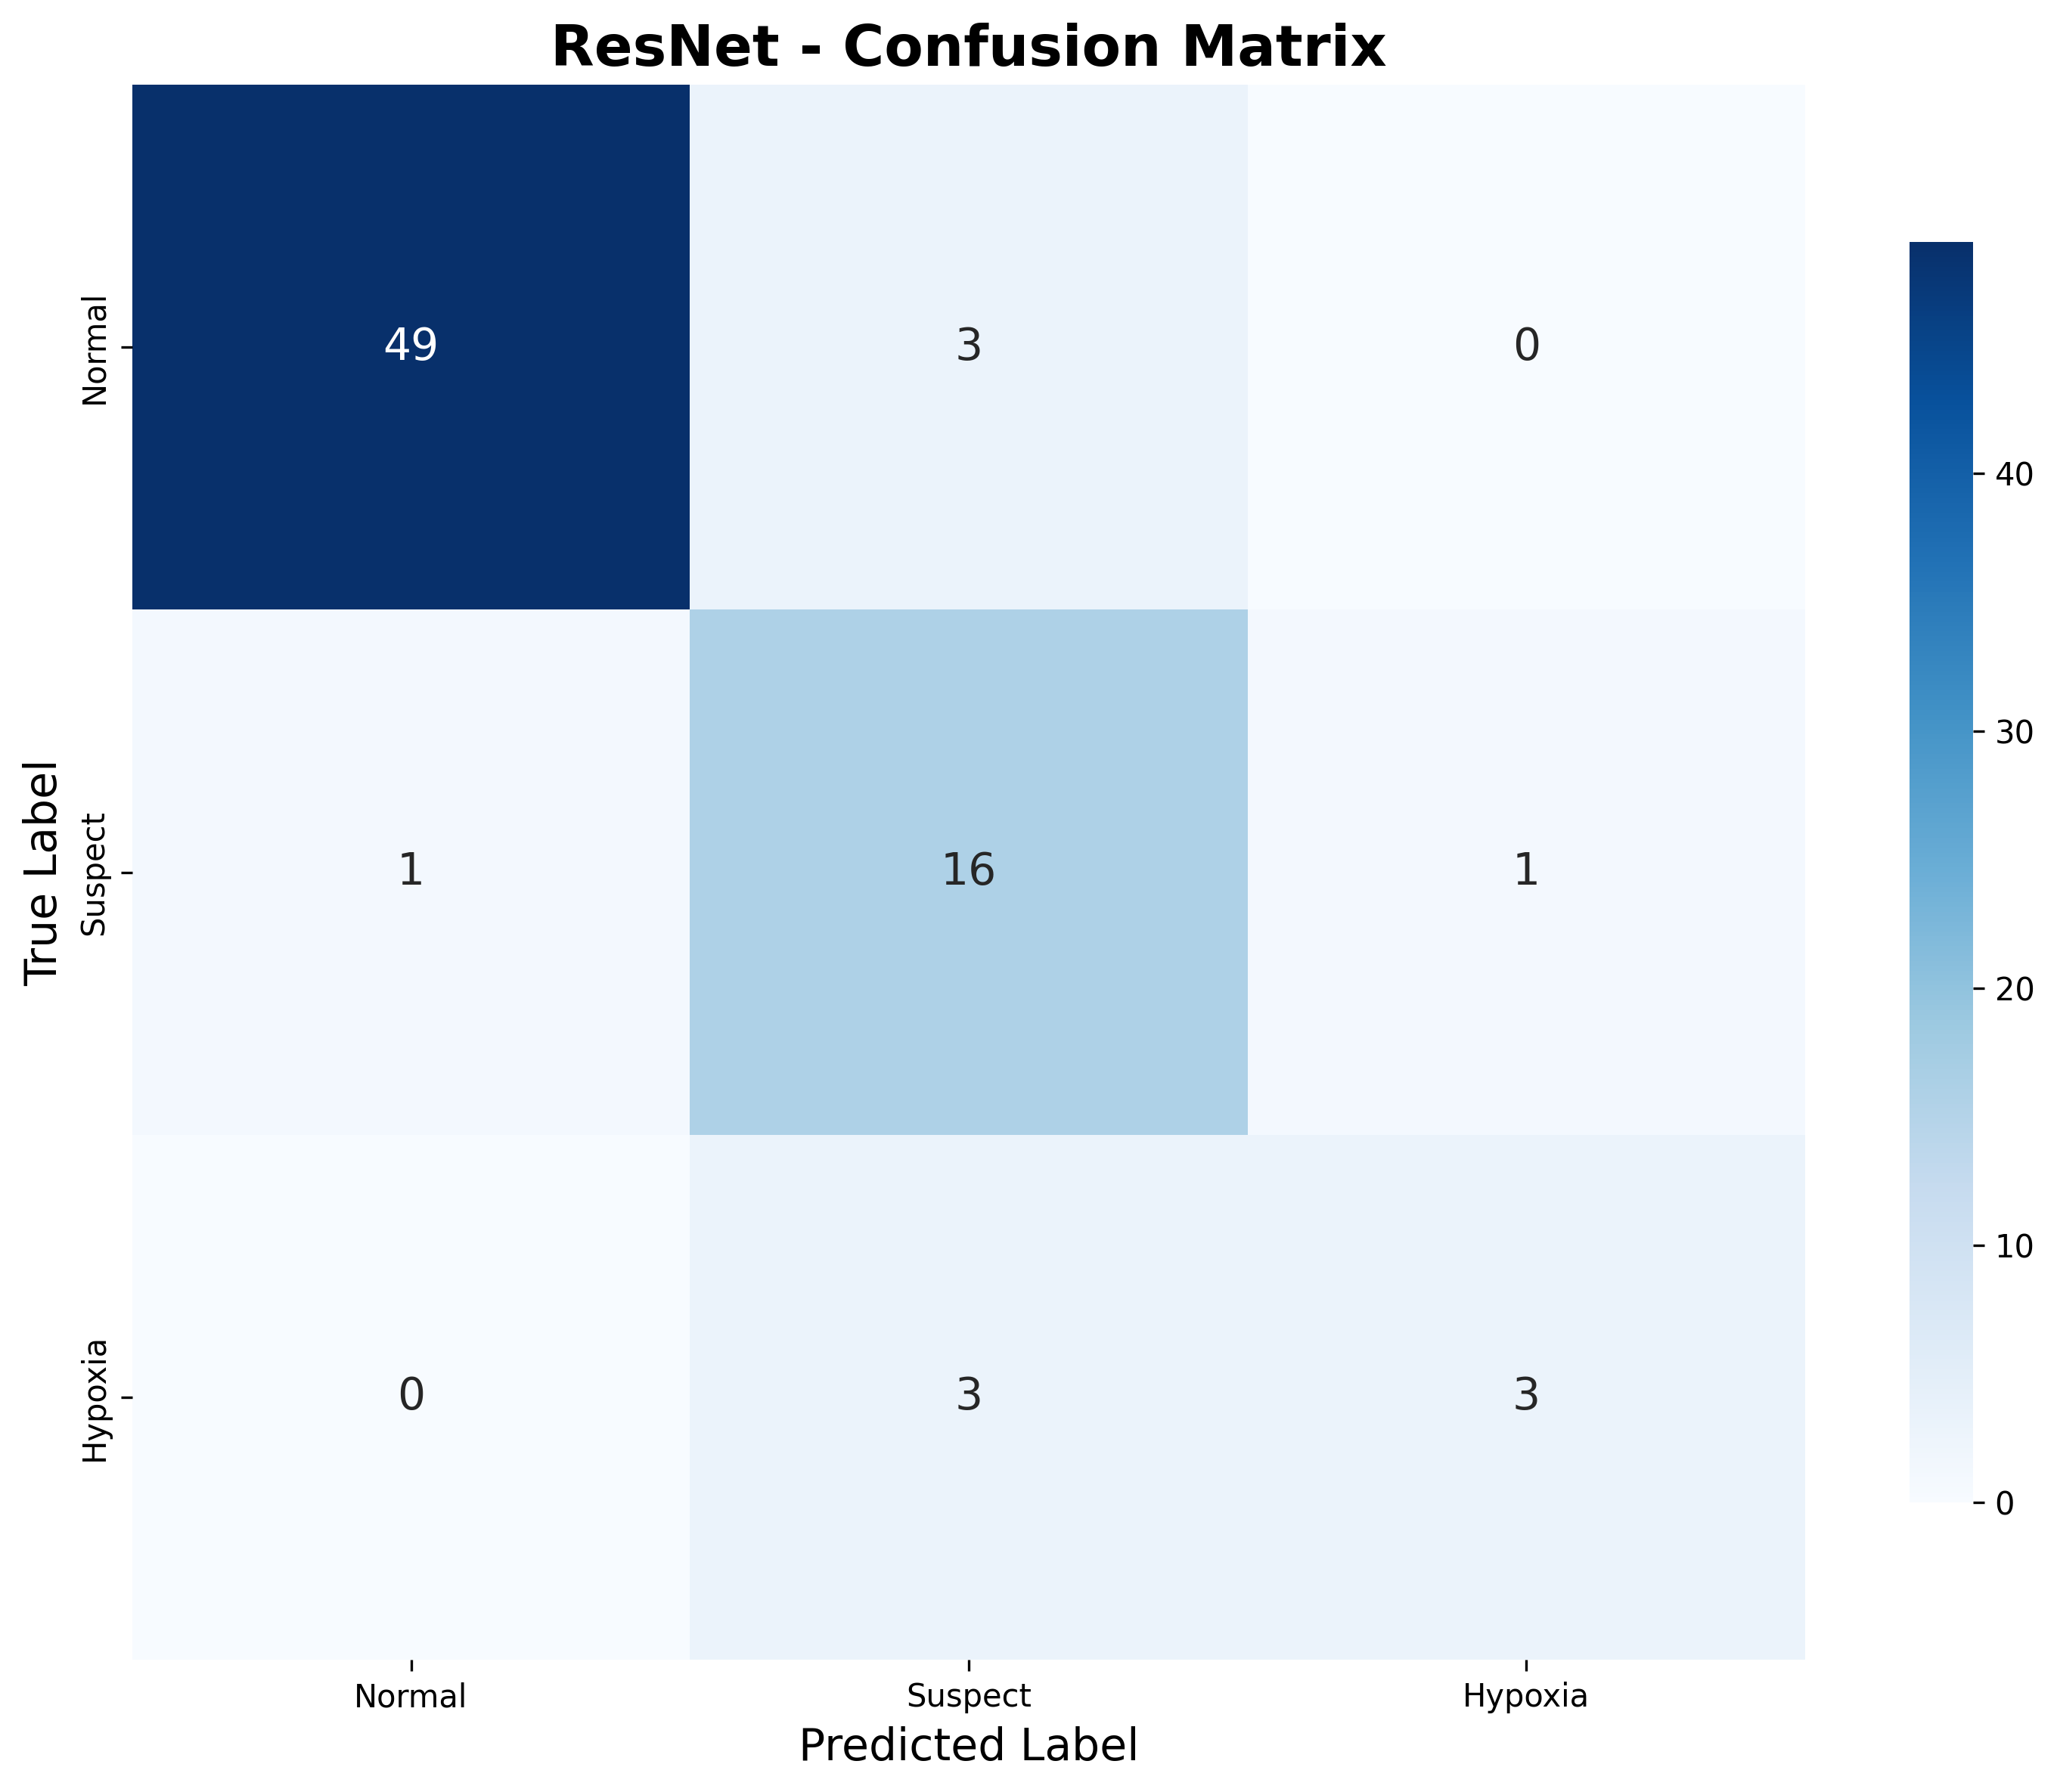
\includegraphics[width=0.85\textwidth]{../results/training_plots/trainingResultResNetMethod/03_confusion_matrix.png}
    \caption{Confusion matrix pada data uji untuk klasifikasi tiga kelas.}
    \label{fig:confusion-matrix}
\end{figure}

\begin{figure}[H]
    \centering
    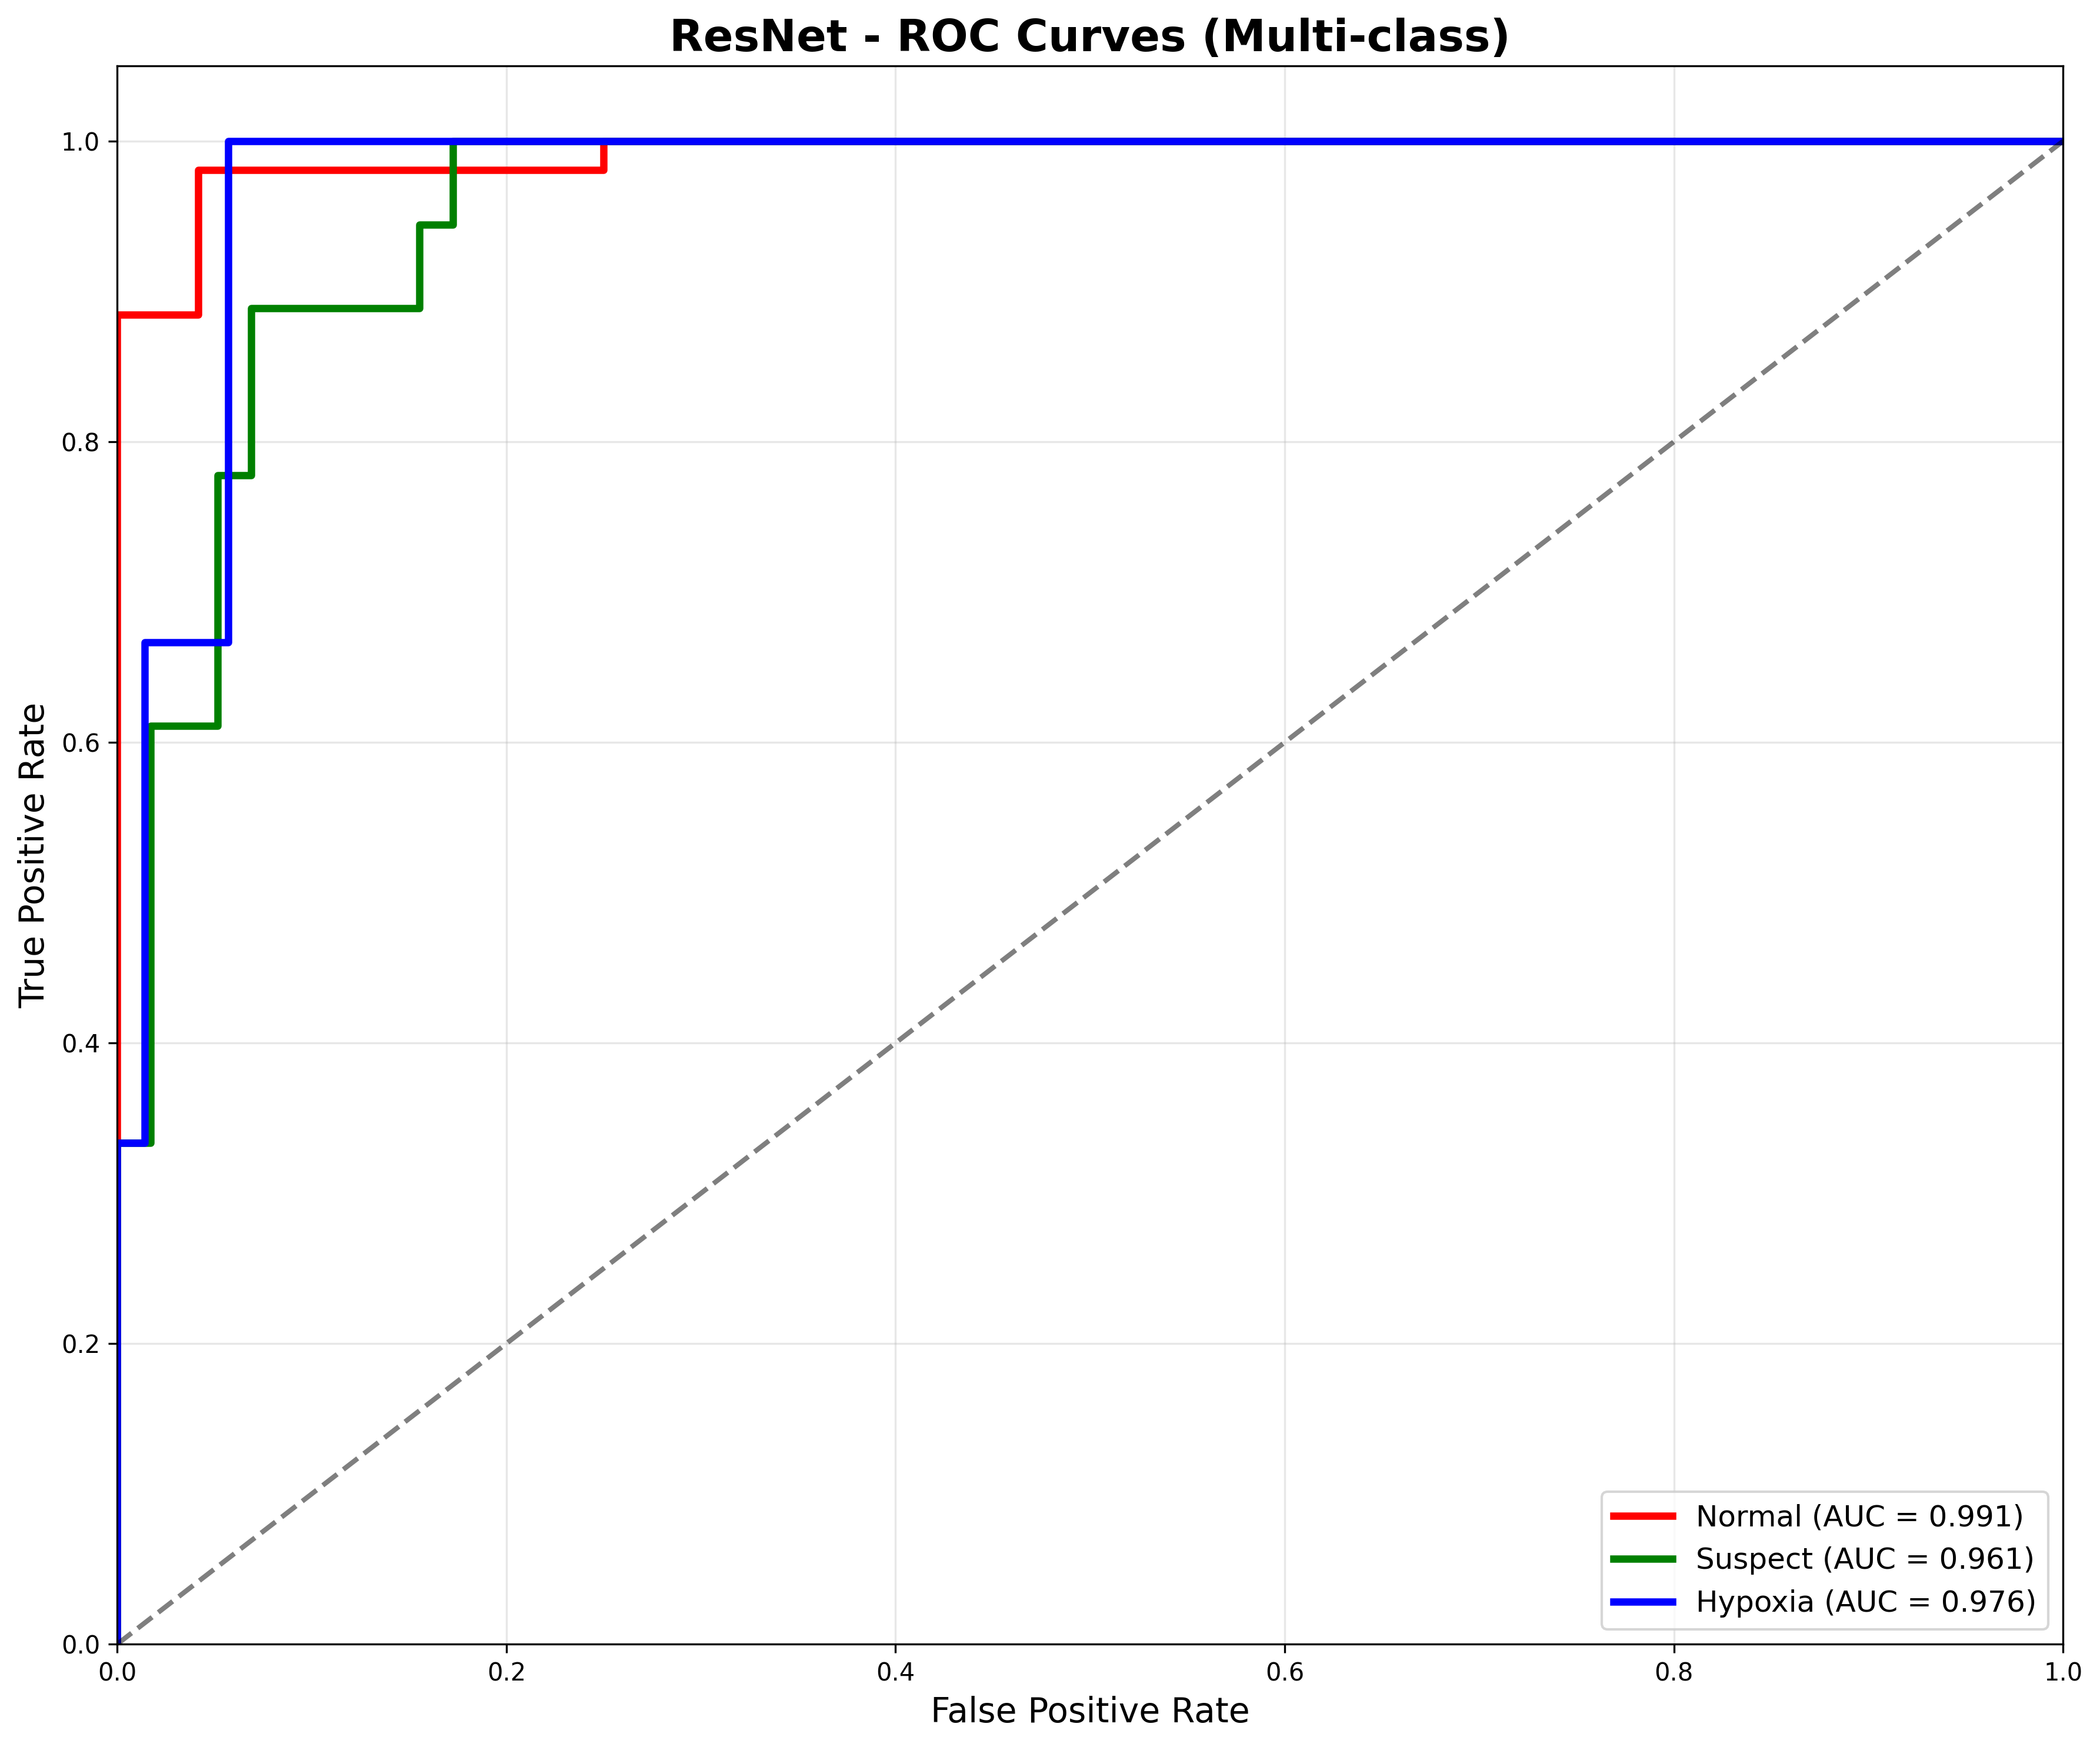
\includegraphics[width=0.85\textwidth]{../results/training_plots/trainingResultResNetMethod/04_roc_curves.png}
    \caption{Kurva ROC multi-kelas yang menunjukkan sensitivitas model untuk tiap label.}
    \label{fig:roc-curves}
\end{figure}

\begin{figure}[H]
    \centering
    \includegraphics[width=0.85\textwidth]{../results/prediction_analysis/predictionResultResNetMethod/03_prediction_summary.png}
    \caption{Ringkasan probabilitas prediksi ResNet pada salah satu rekaman uji.}
    \label{fig:prediction-summary}
\end{figure}

\begin{figure}[H]
    \centering
    \includegraphics[width=0.85\textwidth]{../results/prediction_analysis/predictionResultResNetMethod/07_feature_importance.png}
    \caption{Kontribusi relatif fitur klinis dalam prediksi hipoksia.}
    \label{fig:prediction-importance}
\end{figure}

\begin{figure}[H]
    \centering
    \includegraphics[width=0.85\textwidth]{../results/prediction_analysis/predictionResultResNetMethod/09_uncertainty_analysis.png}
    \caption{Analisis ketidakpastian model untuk kasus uji yang sama.}
    \label{fig:prediction-uncertainty}
\end{figure}

\section{Bab 4: Hasil dan Pembahasan}
\subsection{Hasil Pelatihan}
Model berhenti pada epoch ke-80 dengan \textit{val accuracy} 0.8816 dan laju belajar 7.5\,\texttimes\,10\textsuperscript{-5}. Akurasi uji mencapai 0.7895 dengan loss 0.4310; \textit{precision/recall} kelas normal 0.98/0.85, suspect 0.54/0.72, dan hipoksia 0.43/0.50. Macro F1 0.66 menegaskan tantangan pada kelas minor, sementara \textit{weighted} F1 0.80 menunjukkan performa keseluruhan yang solid.

\subsection{Analisis Kinerja}
Kurva pada Gambar~\ref{fig:training-loss} dan Gambar~\ref{fig:training-accuracy} menunjukkan konvergensi stabil tanpa indikasi \textit{overfitting}. ROC multi-kelas pada Gambar~\ref{fig:roc-curves} menegaskan area tinggi untuk kelas normal, sementara kelas hipoksia masih membutuhkan peningkatan recall melalui augmentasi segmental atau pengaturan ulang bobot kelas. Distribusi kepercayaan model memperlihatkan cluster tajam untuk kelas normal tetapi lebih menyebar pada kelas hipoksia, menandakan perlunya strategi peningkatan sensitivitas.

\subsection{Analisis Prediksi Individual}
Panel interpretasi pada Gambar~\ref{fig:prediction-summary}, Gambar~\ref{fig:prediction-importance}, dan Gambar~\ref{fig:prediction-uncertainty} menampilkan probabilitas tiap kelas, pentingnya fitur klinis (misalnya pH dan usia gestasi), serta analisis ketidakpastian. Fitur klinis dengan kontribusi tinggi berkorelasi dengan pola FHR yang terdeteksi dalam cabang sinyal. Pendekatan multimodal ini sejalan dengan prinsip XAI pada domain medis\textsuperscript{[7]}.

\subsection{Implikasi Klinis}
Integrasi sinyal dan metadata klinis mengurangi risiko ketergantungan pada satu sumber informasi. Panel visual memungkinkan dokter kandungan meninjau kepercayaan model sebelum memutuskan intervensi, sehingga sistem dapat diposisikan sebagai \textit{clinical decision support} yang memperkuat praktik obstetri.

\subsection{Keterbatasan}
Ukuran kelas hipoksia yang kecil menyebabkan interval kepercayaan recall relatif lebar. Evaluasi terbatas pada satu sumber data (CTU-UHB) sehingga generalisasi perlu diuji di rumah sakit lain. Selain itu, sinyal kontraksi uterus belum dimodelkan secara eksplisit.

\section{Bab 5: Kesimpulan dan Saran}
\subsection{Kesimpulan}
\begin{enumerate}[label=\arabic*)]
    \item Pipeline konversi \texttt{.dat/.hea} ke \texttt{.npy} dan tabular klinis berhasil menghasilkan 506 sampel valid dengan 27 fitur numerik siap latih.
    \item Arsitektur ResNet multimodal dengan residual projection, \textit{global pooling}, fusi atensi, dan cabang klinis terstandar memberikan kerangka matematis yang stabil untuk sinyal panjang.
    \item Evaluasi menunjukkan akurasi 0.7895 dan \textit{weighted} F1 0.80 dengan recall hipoksia 0.50; performa ini memadai sebagai prototipe klinis yang mengutamakan sensitivitas terhadap kasus kritis.
    \item Panel visual dan analisis prediksi meningkatkan interpretabilitas serta selaras dengan rekomendasi literatur mengenai transparansi model medis.
\end{enumerate}

\subsection{Saran}
\begin{enumerate}[label=\arabic*)]
    \item Melakukan validasi eksternal pada rumah sakit berbeda untuk mengakomodasi variasi instrumentasi CTG dan populasi pasien.
    \item Menambahkan blok residual tambahan atau attention temporal adaptif guna meningkatkan recall hipoksia tanpa menurunkan akurasi kelas normal.
    \item Mengintegrasikan teknik XAI berbasis atensi segmental agar segmen FHR paling informatif dapat ditinjau cepat oleh klinisi.
    \item Menerapkan protokol hibrida: ResNet sebagai triage awal diikuti telaah manual bagi kasus suspect/hipoksia dengan \textit{confidence} rendah.
\end{enumerate}

\subsection{Rencana Penelitian Lanjutan}
\begin{enumerate}[label=\arabic*)]
    \item Mengembangkan modul inferensi real-time berbasis \textit{edge computing} dan menilai performanya di ruang bersalin.
    \item Mengeksplorasi fungsi kerugian hibrida (focal + dice) untuk menyesuaikan trade-off precision--recall sesuai kebutuhan klinis.
    \item Menambahkan sinyal kontraksi uterus serta fitur \textit{time-to-event} dari header \texttt{.hea} sebagai kovariat baru dalam model.
\end{enumerate}

\section*{Ucapan Terima Kasih}
Tim mengapresiasi ketersediaan database CTU-UHB di PhysioNet serta komunitas \textit{open-source} TensorFlow dan scikit-learn yang mendukung pengembangan pipeline ini.

\section*{Daftar Pustaka}
\begin{enumerate}[label={[\arabic*]}]
    \item K. Chudáček et al., ``Open access intrapartum CTG database,'' \textit{BMC Pregnancy and Childbirth}, vol. 14, p. 16, 2014.
    \item C. W. G. Redman and P. Georgieva, ``Computerized interpretation of fetal heart rate patterns,'' \textit{BJOG}, vol. 116, pp. 2--10, 2009.
    \item K. He, X. Zhang, S. Ren, and J. Sun, ``Deep residual learning for image recognition,'' in \textit{Proceedings of the IEEE Conference on Computer Vision and Pattern Recognition}, 2016, pp. 770--778.
    \item R. Dey and F. M. Salemt, ``Residual convolutional neural network for ECG signal classification,'' in \textit{IEEE EMBS BHI}, 2017, pp. 1--4.
    \item T.-Y. Lin, P. Goyal, R. Girshick, K. He, and P. Dollár, ``Focal loss for dense object detection,'' in \textit{Proceedings of the IEEE International Conference on Computer Vision}, 2017, pp. 2999--3007.
    \item D. M. W. Powers, ``Evaluation: From precision, recall and F-measure to ROC, informedness, markedness and correlation,'' \textit{Journal of Machine Learning Technologies}, vol. 2, pp. 37--63, 2011.
    \item M. Tjoa and C. Guan, ``A survey on explainable artificial intelligence (XAI) for deep learning,'' \textit{Information Fusion}, vol. 67, pp. 1--25, 2021.
    \item A. Georgieva et al., ``Computer-based analysis of intrapartum fetal heart rate monitoring: a systematic review,'' \textit{PLoS ONE}, vol. 14, no. 7, e0218131, 2019.
\end{enumerate}

\end{document}
